\chapter{Example}\label{sec:example}

\section{Brain Sources Localization}\label{sec:BSL_example}
%\lstinputlisting{../../misc/demo/Brain_source_localization/BSL.m}



\paragraph{} An experience of Brain Source Localization using several gain matrices including FA$\mu$ST and several solvers is provided. After configuring the Matlab path (cf section \ref{sec:firstUseMatlabPath}), you can execute the Matlab script: \\
\texttt{/<HOMEDIR>/Documents/MATLAB/Faust/demo/Brain\_source\_localization/BSL.m}\\
to run this experiment and the file:\\
\texttt{/<HOMEDIR>/Documents/MATLAB/Faust/demo/Brain\_source\_localization/Fig\_BSL.m} \\
to display the following pictures illustrating the speed-up using a FA$\mu$ST.\\
In the Matlab Command Window, you just need to type :
\begin{lstlisting}
>> BSL
>> Fig_BSL
\end{lstlisting}

Which allows you to visualize this figure illustrating the speed-up with a FA$\mu$ST ($\mathbf{M}$ is the gain dense matrix and $\widehat{\mathbf{M}}_{6},\widehat{\mathbf{M}}_{9},\widehat{\mathbf{M}}_{16},\widehat{\mathbf{M}}_{26}$ are different FA$\mu$ST representing  $\mathbf{M}$):

\begin{figure}[!htbp]
\label{fig:BSL}
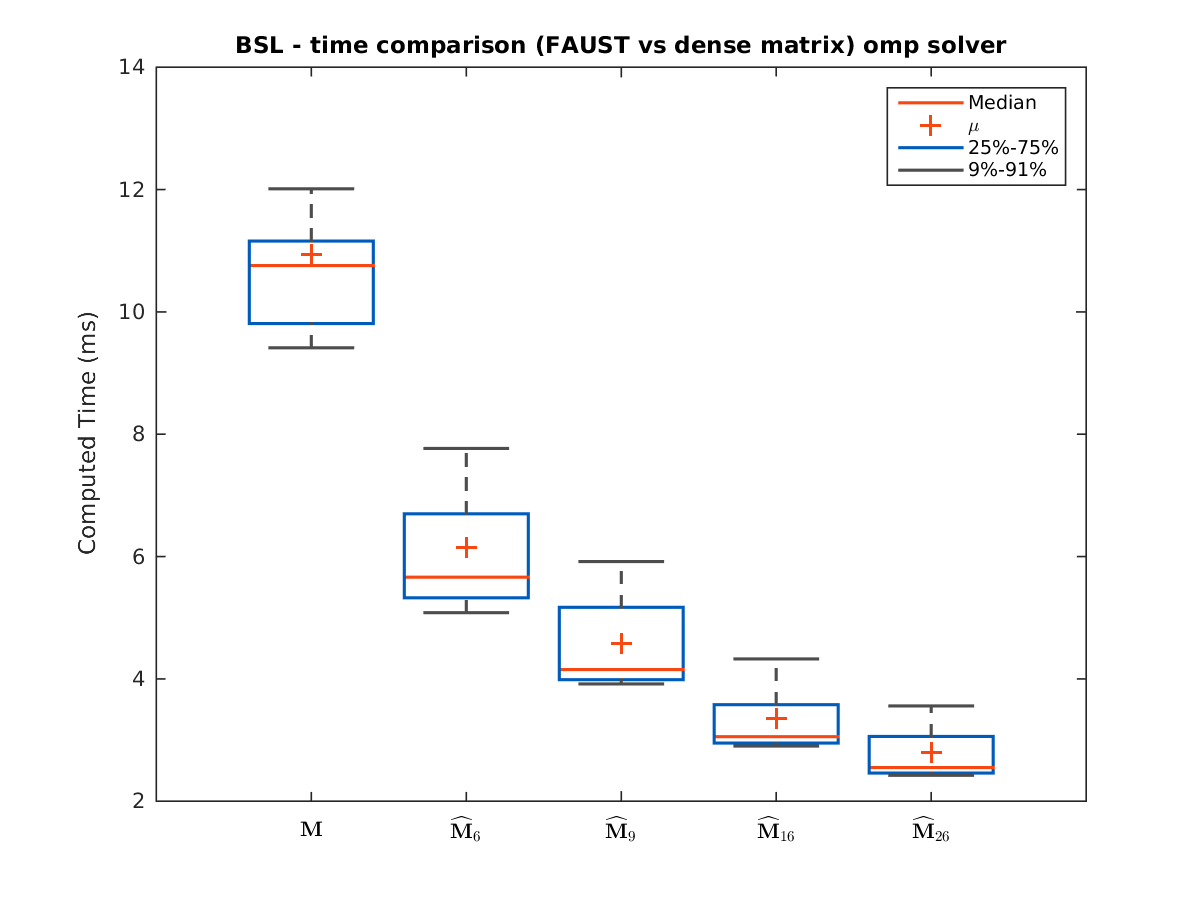
\includegraphics[scale=0.7]{images/BSL.png}
\end{figure}
